%----------------------------------------------------------------------------
\label{Pockels cell pulse section}
%----------------------------------------------------------------------------
%----------------------------------------------------------------------------
%----------------------------------------------------------------------------
%bb defines the bounding box for the pdf
%viewport defines the area of the pdf used
%in sidewaysfigure the last entry in bb moves the caption toward/away the pic
%in sidewaysfigure the second entry in bb moves the pic toward/away the caption
%----------------------------------------------------------------------------
\begin{figure}
\scalebox{0.68}[0.68]{
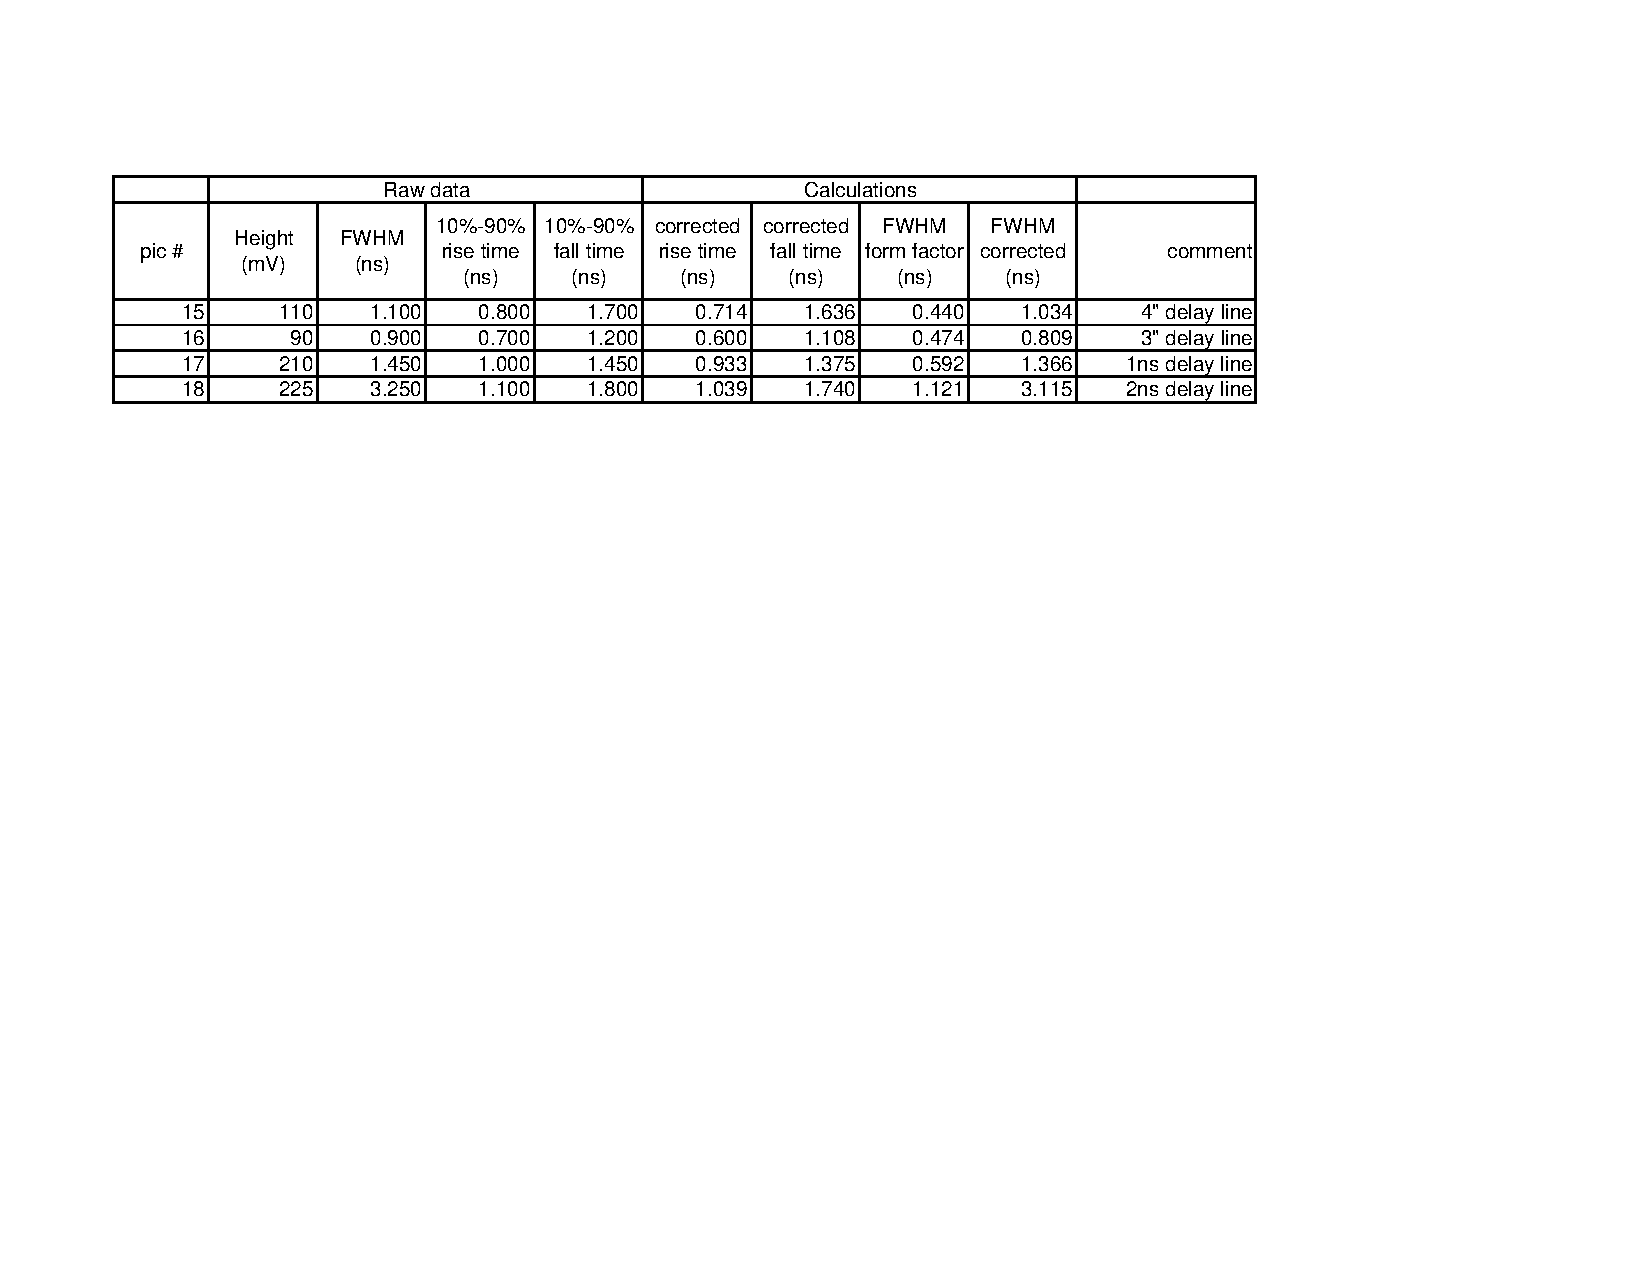
\includegraphics[bb=10 400 605 550]
{delay_lines/delay_lines.pdf}
}
\caption[Pulse length data/calculation table]{Pulse length data/calculation table. Data resulting from various delay lines are corrected for the limited temporal properties of the data acquisition system. The 1ns delay line is 7 7/8'' long and the 2ns delay line is 15 3/4'' long (from connector tip to connector tip).}
\label{delay lines}
\end{figure}
%----------------------------------------------------------------------------

%----------------------------------------------------------------------------
The dye laser generates 535.892nm output (held within 2 picometers by the ``LambdaLok'' feature of the dye laser) at 20Hz with 5ns pulse lengths using a Coumarin 153 dye pumped with a tripled Nd:YAG (355nm) beam. In order to shape the pulsed dye laser output with the Pockels cell, the YAG pump is synchronized with the Hg pulser (which runs the Pockels cell) so that the cell activates at the exact same time the dye laser pulse traverses the crossed polarizers (in the case of the dye laser, we use two polarizing cube beam splitters from Lambda Research Optics) and the cell. This is accomplished through the use of three HP 8015A pulse generators and a few delay lines. Pulser \#1 is designated the ``clock generator'' and triggers the Hg pulser and the flashlamps in the YAG.

%----------------------------------------------------------------------------
%----------------------------------------------------------------------------
%bb defines the bounding box for the pdf
%viewport defines the area of the pdf used
%in sidewaysfigure the last entry in bb moves the caption toward/away the pic
%in sidewaysfigure the second entry in bb moves the pic toward/away the caption
%----------------------------------------------------------------------------
\begin{figure}
\scalebox{0.8}[0.8]{
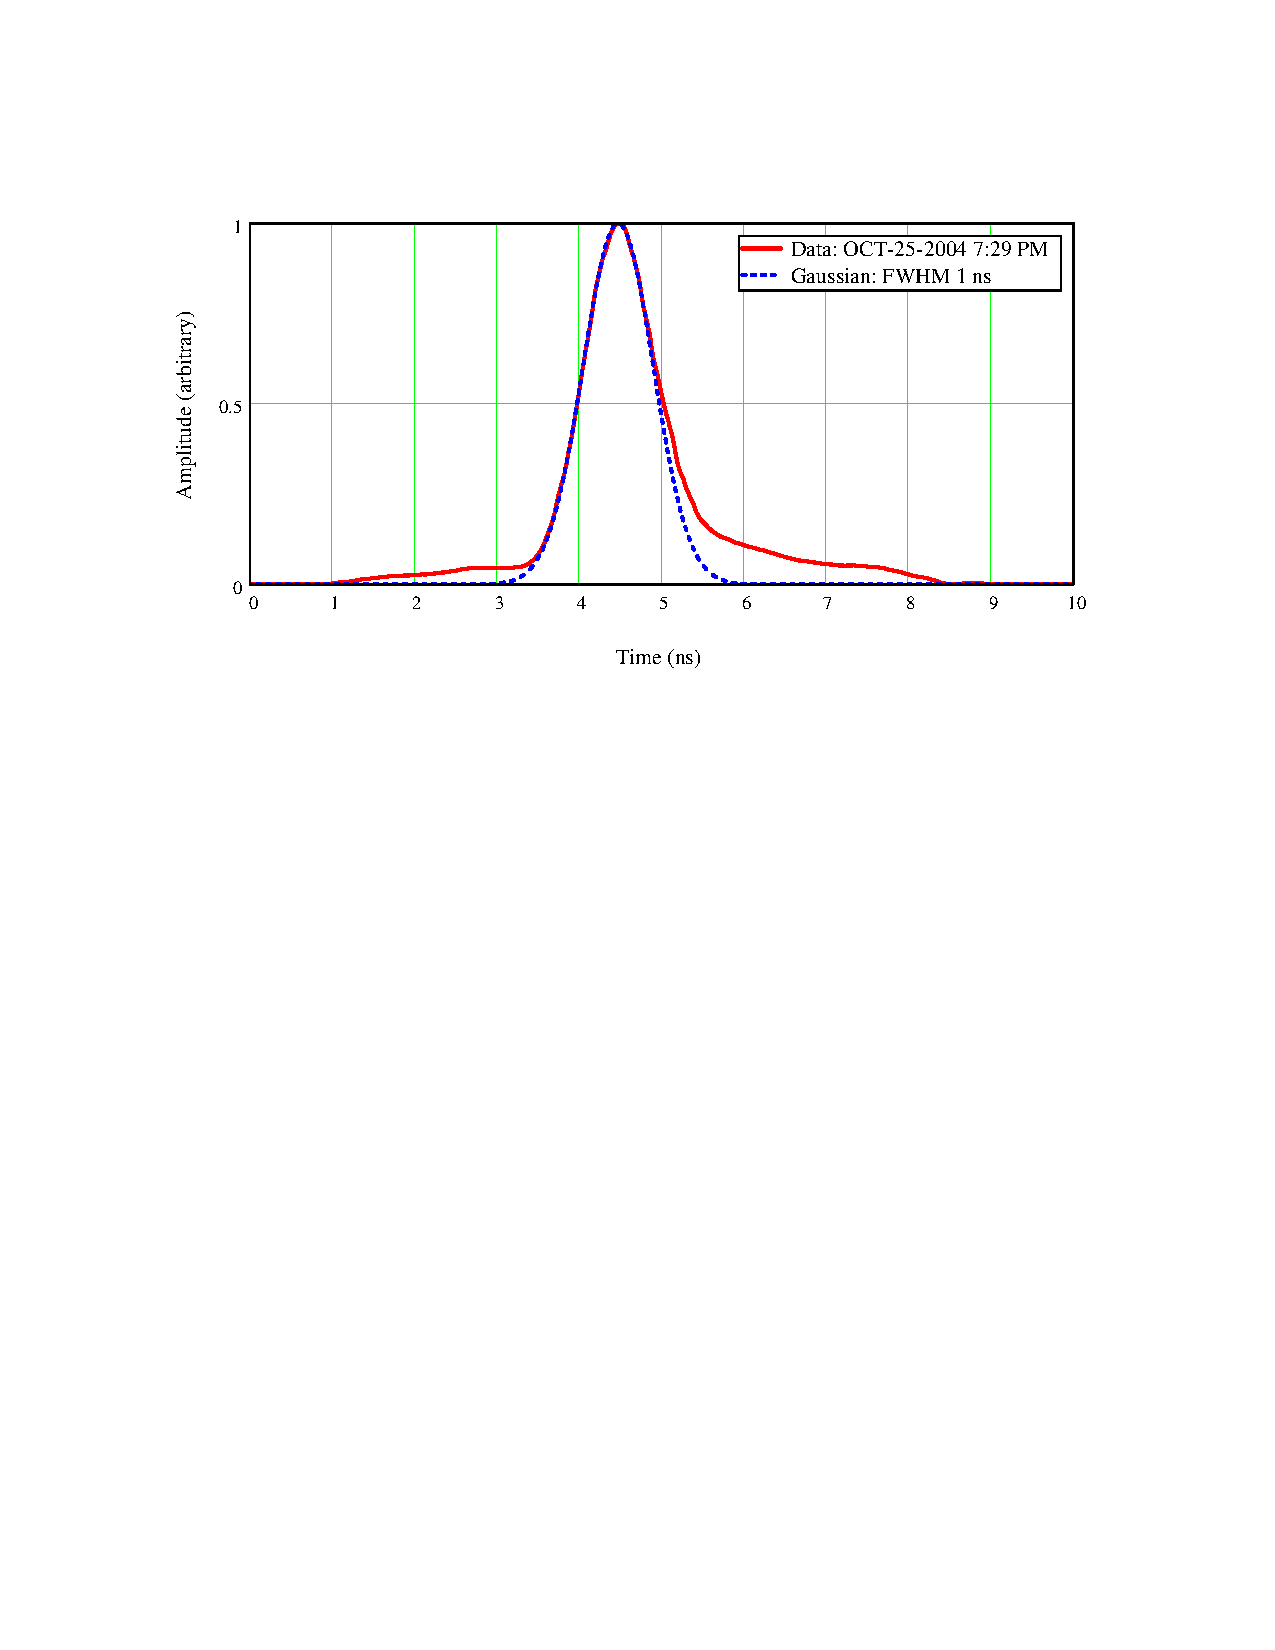
\includegraphics[bb=35 467 523 689]
{temporal_profiles/temporal_profiles.pdf}
}
\caption[Pockels cell minimum pulse length (temporal profiles)]{Pockels cell minimum pulse length (temporal profiles). Here the data corresponding to a 3'' delay cable is overlaid with a computer generated Gaussian pulse. There is significant leaking before and after the pulse; this perhaps due to the relatively low (manufacturer specified) extinction ratio of 1k:1 for the polarizers (compared to 10k:1 for the polarizers used in the HeNe test) and the mismatch between the design wavelength and the laser wavelength.}
\label{temporal profiles}
\end{figure}
%----------------------------------------------------------------------------

%----------------------------------------------------------------------------
The trigger signal for the Hg pulser is sent directly while the TTL trigger signal for the flashlamps is delayed in pulser \#2 (designated the ``flashlamp delay generator'') by about 1060$\mu$s. This flashlamp delay is varied so that the Q-switch opens near the peak of the flashlamp induced population inversion in the Nd:YAG rods; in our case this was about 340$\mu$s before the Q-switch delay generator (see below) TTL pulse. Upon receiving the trigger signal from the clock generator, the Hg pulser closes in about 1.4ms: the high voltage output pulse is to the Pockels cell through 220' of coax cable (introducing a fixed delay of 300ns) while the trigger output is sent to the Q-switch in the YAG.

%----------------------------------------------------------------------------
%----------------------------------------------------------------------------
%bb defines the bounding box for the pdf
%viewport defines the area of the pdf used
%in sidewaysfigure the last entry in bb moves the caption toward/away the pic
%in sidewaysfigure the second entry in bb moves the pic toward/away the caption
%----------------------------------------------------------------------------
\begin{figure}
\scalebox{0.8}[0.8]{
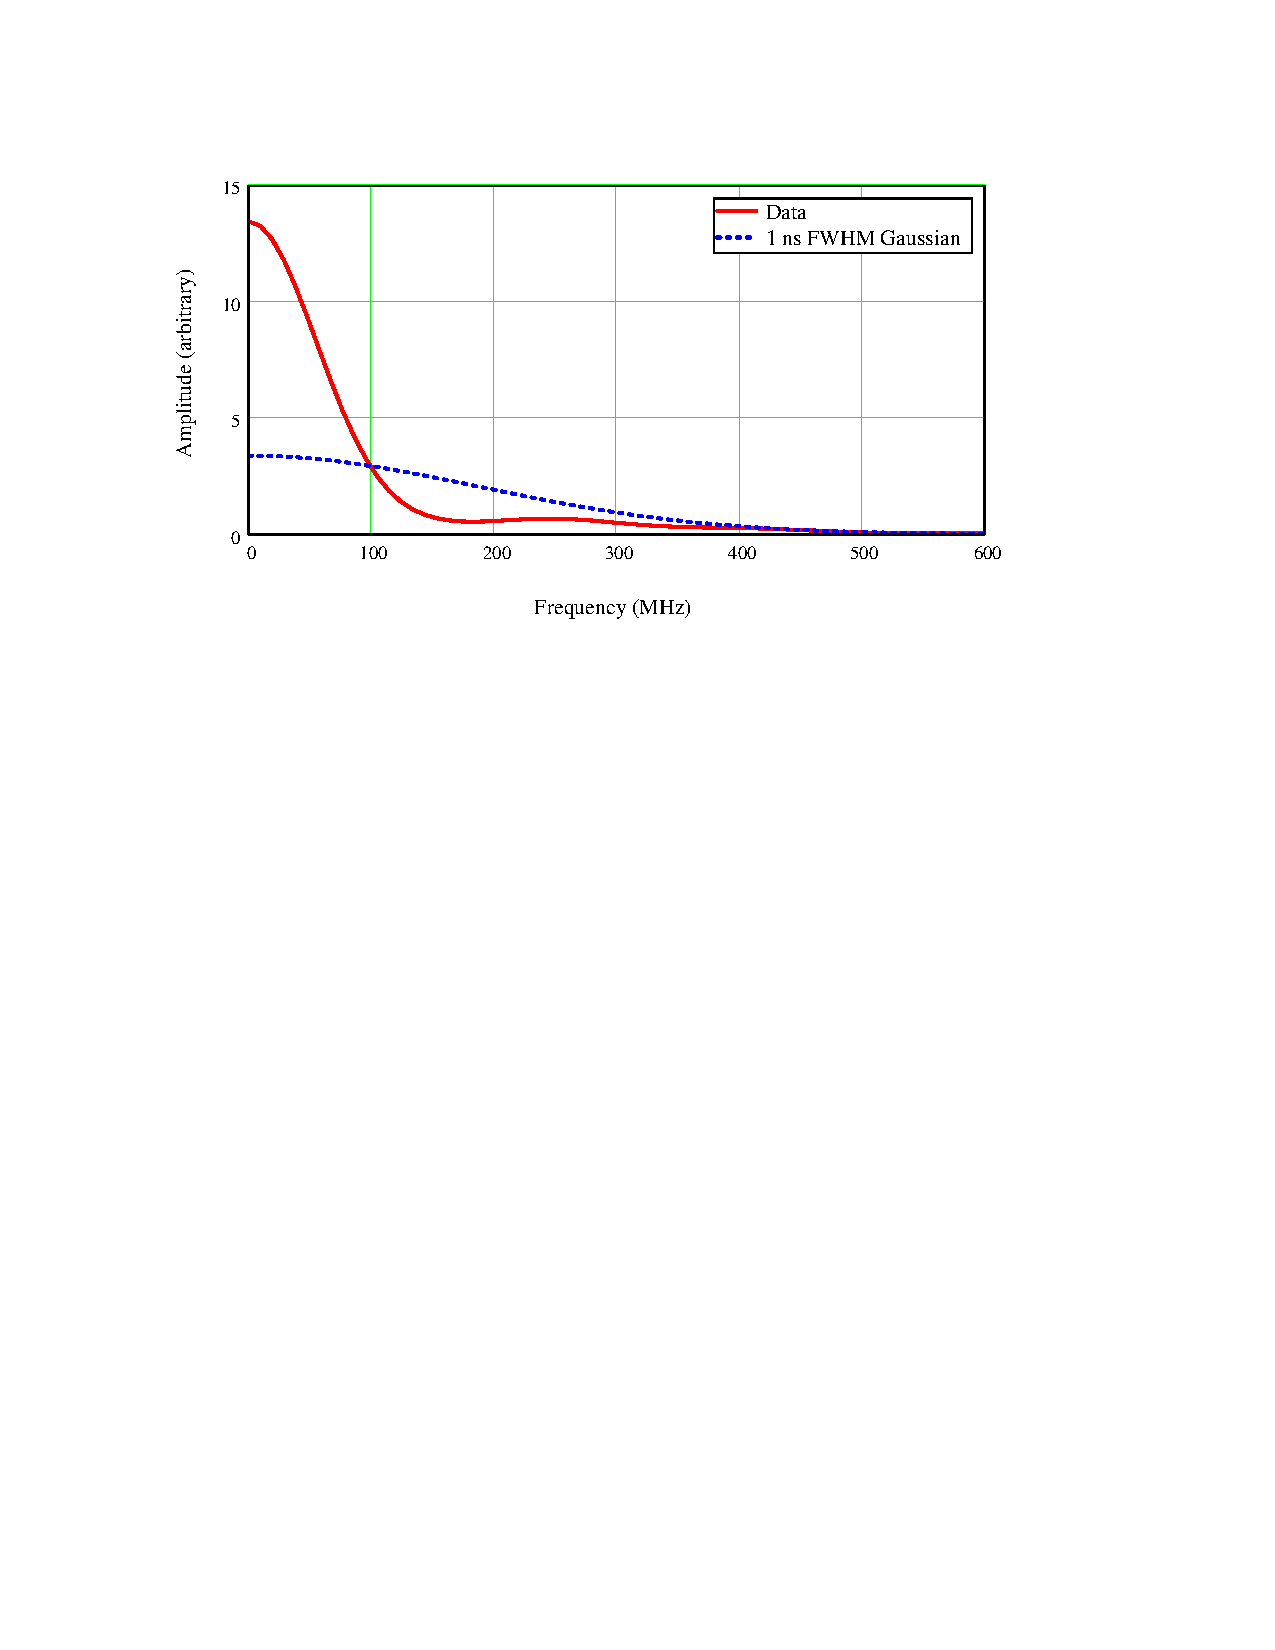
\includegraphics[bb=20 494 481 690]
{spectral_profiles/spectral_profiles.pdf}
}
\caption[Pockels cell minimum pulse length (spectral profiles)]{Pockels cell minimum pulse length (spectral profiles). The power spectrum of the pulses in Figure \ref{temporal profiles} (from a FFT of the temporal profiles) are show here. The leaking results in significant distortion from the optimal Gaussian profile.}
\label{spectral profiles}
\end{figure}
%----------------------------------------------------------------------------

%----------------------------------------------------------------------------
On its way to the YAG's Q-switch input, the trigger signal from the Hg pulser is first sent through a 20dB attenuator and then through pulser \#3 designated the ``Q-switch delay generator'', which adds about 200ns of variable delay. This TTL delay pulse is adjusted to that the subsequent dye laser pulse (the activated Q-switch generates a YAG pulse which in turn generates a dye laser pulse) arrives at the Pockels cell at the exact moment the Pockels cell is activated; in our case this was about 80ns before the Pockels cell is activated. A paper target is placed at the output of the optical switch and the scattered light from the target is observed using a fast photodiode (Electro-optics ET-2000).

For the Hg pulser, a delay line controls the pulse length. The high voltage output pulse is split: half of the signal is sent to the Pockels cell while the other half is sent down an un-terminated (delay line) cable. The high voltage rise reflects inverted from the open end of the cable and returns to cancel the signal sent to the Pockels cell -- this terminates the voltage signal. Thus, the height of the output pulse is half the charging line voltage. Moreover, the pulse length is twice the delay line travel time and the falling edge should have a similar shape as the rising edge. In fact the falling edge shape will always be a distorted version of the rising edge shape due to the inherent frequency dependent attenuation and phase shift introduced by the losses in real cables. We are able to produce fairly symmetric looking pulses out to 200 ns using typical coaxial cable as a delay line.

To determine the minimum pulse length obtainable, a 7'' delay line is successively shortened (using wire cutters) by 1'' increments and the resulting laser pulses at each length are observed on a Tektronix 7104 oscilloscope. The pulse images are recorded using a Polaroid camera attachment for the scope. The Polaroid prints were then analyzed with dividers and a straight edge to determine the height (in mV), the rise and fall times (in ns), and the FWHM (in ns) of each photographed trace. Given the rise/fall time of the photodiode (200/350ps) and the rise/fall time of the oscilloscope (300ps), the rise/fall time and FWHM measurements from the Polaroid images can be corrected using the following formulae
%----------------------------------------------------------------------------
\begin{equation}
t_{r}^2
=
\tau_{r}^2
+
p_{r}^2
+
s_{rf}^2,
\end{equation}
%----------------------------------------------------------------------------
%----------------------------------------------------------------------------
\begin{equation}
t_{f}^2
=
\tau_{f}^2
+
p_{f}^2
+
s_{rf}^2,
\end{equation}
%----------------------------------------------------------------------------
%----------------------------------------------------------------------------
\begin{equation}
t_{w}
=
f_{w}
(t_{r} + t_{f}),
\end{equation}
%----------------------------------------------------------------------------
and
%----------------------------------------------------------------------------
\begin{equation}
\tau_{w}
=
f_{w}
(\tau_{r} + \tau_{f})
\end{equation}
%----------------------------------------------------------------------------
where $p_{r}$ is the photodiode rise time, $p_{f}$ is the photodiode fall time, $p_{r}$ is the photodiode rise time, $s_{rf}$ is the Tektronix 7104 rise/fall time, $t_{r}$ is the measured rise time, $t_{f}$ is the measured fall time, $t_{w}$ is the measured FWHM, $\tau_{r}$ is the corrected rise time, $\tau_{f}$ is the corrected fall time, $f_{w}$ is the FWHM form factor, and $\tau_{w}$ is the corrected FWHM.

We found that a 3'' delay cable produced the best results; see Figure \ref{delay lines} for a data/calculation table. To determine the degree to which the output pulse approximates a Gaussian, a power spectrum of the (uncorrected) temporal envelope is calculated. See Figure \ref{temporal profiles} and \ref{spectral profiles} for the results. It is found that ``leaking'' caused by poor polarizer extinction ratios can significantly distort the power spectrum profile from the Gaussian case.
%----------------------------------------------------------------------------
%----------------------------------------------------------------------------
